\section{Evaluation}
\par Throughout the project, we have made several
decisions over the representations of mathematical objects such as
subsets. We will disucss their consequences in this
section. Furthermore, we will also review the whole development process. At the end of this section, we
will also discuss the feasibility of formalising mathematics and
programming logic in practice. 


\subsection{Different choices of representations}
\par In computer proofs, an abstract mathematical
object usually requires a concrete representation. Different representations will lead to different
formalisations and thus contribute to the
easiness or difficulty in completing the proofs. In the
following paragraphs, we will discuss the representations we have
chosen and their consequences. 

\paragraph{The set of states (Q) and its subsets} As we have mentioned
in section 3, Firsov and Uustalu \cite{firsov2013} represent the set of states (\mb{Q}) and its subsets
as column vectors. However, this representation looks unnatural compare
to the actual mathematical definition. Therefore, at the beginning, we intended to avoid the vector representation and to
represent the sets in abstract forms. In our approach, the set of states is represented as a data type in Agda, i.e. \mb{Q : Set}, and its
subsets are represented as unary functions on \mb{Q}, i.e. \mb{DecSubset\ Q = Q \to
  Bool}. 

\par Our definition allows us to finish the proofs in
\textbf{Correctness/RegExp-eNFA.agda} without having to
manipulate matrices. The proofs also look much more natural compare to that in
\cite{firsov2013}. However, problems arise when the sets have to be iterated when computing the 
\(\epsilon\)-closures because it is impossible to iterate the sets
using this representation. In order to solve the problems, several
extra fields are added into the definition of automata such as \mb{It}
-- a vector containing all the states in \mb{Q}. With \mb{It}, a subset
of \mb{Q} can be iterated by applying it own function, \mb{Q \to
  Bool}, to all the elements in \mb{It}. Note that the vector \mb{It}
is equivalent to the vector representation of \mb{Q}. 

\paragraph{The accepting languages of regular expressions and finite automata} At first, the
accepting language of regular expression was defined as a decidable
subset, i.e. \(L^R : RegExp \to DecSubset\ \Sigma^*\). The decision
was reasonable because the language has been proved decidable for many
years. However, \(L^R\) is also a boolean decider for regular
expressions and this definition added a great amount of
difficulties in writing the proofs because the proofs had to be built
on top of the decider. For example, in the concatenation case, an extra recursive
function was needed to iterate different combinations of input
string and correctness proof of this function is difficult to
complete. However, the decidability of the languages is actually not
necessary in proving their equality. Therefore, in the current version
of our Agda code, the language is defined using the general subset, i.e. \mb{L^R : RegExp \to Subset\
  \Sigma^*}. This definition allows to prove the equality of the languages
in an abstract level. 

\par The same situation also applies to the accepting language of finite automata. At first, the
accepting language of NFA was obtained by running an algorithm that
produces all the reachable states from \mb{q_0} using the input
string. The algorithm was also a decider for NFA. Once again, this
definition mixes the decider and the proposition together. Therefore,
the accepting language of NFA is now defined in an abstract form. 

\par However, this does not mean that we can ignore all the algorithms. In
fact, we still need to design algorithm in computing \(\epsilon\)-closures and
powerset construction. Here is our approach: 1) separate the algorithm from the
mathematical definition and 2) prove that they are equivalent. In this
way, the decidability of the mathematical definition will follow from that
of the algorithm. The advantage is that it is easier to use the
abstract mathematical definition in other proofs than using the algorithm. 

\paragraph{The set of reachable states from \(q_0\)} Let us recall the
definition of reachable states from \mb{q_0}. 
\begin{center} 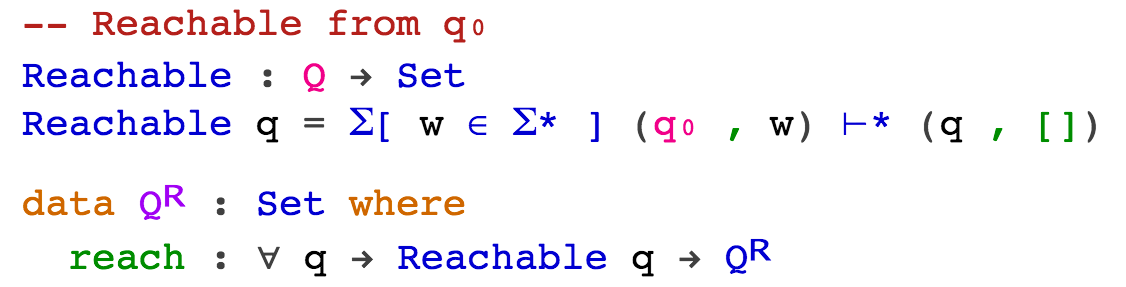
\includegraphics[width=.6\textwidth]{reach} \end{center}

\par We say that a state \mb{q} is reachable if and
only if there exists a string \mb{w} that can take \mb{q_0} to
\mb{q}. Therefore, the set \mb{Q^R} should contains all and only the
reachable states in \mb{Q}. However, there may exist more than one
reachability proof for the same state. Therefore, for a state in \mb{Q}, there may be
more than one element in \mb{Q^R} and thus \mb{Q^R}
may be larger than the original set \mb{Q} or even worse, it may be
infinite. This leads to a problem when a DFA is constructed using
\mb{Q^R} as the set of states. If \mb{Q^R} is
infinite, then it is impossible to iterate the set during 
quotient construction. Even if the set \mb{Q^R} is finite, it
contradicts our original intention to minimise the set of states. This is also one of the
reasons why our formalisation of quotient construction cannot be
completed. However, this has no effects to the proof of \(L(\)DFA\() =
  L(\)MDFA\()\) because we can provide an equality relation of states in
the DFA. In the translation from DFA to MDFA, we defined
the equality relation as follow: any two elements in \mb{Q^R} are equal if and only
if their states are equal. Therefore, two elements with same state
but different reachability proofs are still considered the same in the new DFA. 

\par One possible way to solve the problem is to re-define the
reachability of a state such that any reachable state will have a
unique reachability proof. For example, the representative proof can
be selected by choosing the shortest string \mb{(w)} sorted in
alphabetical order that can take \mb{q_0} to \mb{q}. Another solution is to use
Homotopy Type to declare the set \mb{Q^R}. This type allows us to
group different reachability proofs into a single element such that
every state will only appear once in \mb{Q^R}. 


\subsection{Development Process}
\par As we have mentioned before, the parts related to quotient
construction were not completed. The major reason is
that there was only very limited time left when we started the quotient
construction. In the following paragraphs, we will evaluate the whole
development process and discuss what could have been done better. 

\par In the first 6 weeks, I was struggling to find
the most suitable representations for regular expressions, finite
automata and their accepting languages. During the time, I was
rushing in coding without thinking about the whole picture of
the theory. As a result, many bad decisions had been made; for example, omitting the
\(\epsilon\)-transitions when converting regular expressions to NFA and trying to prove
the decidability of regular expressions directly. After taking the
advice from my supervisor, I followed the definitions in the
book \cite{aho1972} and started to write a framework of the
theory. After that, in just one week, the Agda
codes that formed the basis of the final version were developed by
using the framework. One could argue that the work
done in the first 6 weeks also contribute to those Agda codes but
there is no doubt the written framework highly influenced the
development. Therefore, even though it is convenient to write proofs
using the interactive features in Agda,
it would still be better to start with a framework in early stages. 

\par After that, the development went smooth until the first week of
the second semester. During the time, I started to prove several
properties of \(\epsilon\)-closures. The plan was to finish this part
within 2 weeks. However, 4 weeks were spent on it and very little
progress were made. These 4 weeks were crucial to the development and
the time should have been spent more wisely on other parts of the
project such as powerset construction or the report. 


\subsection{Computer-aided verification in practice}
\par In order to evaluate the feasibility computer-aided verification in
practice, we will discuss: 1) the difference between computer proofs and written proofs, 2) the easiness or
difficulty in formalising mathematics and programming logic and 3) the
difference between computer-aided verification and testing. 


\subsubsection{Computer proofs and written proofs}
\par According to Geuvers \cite{geuvers2009}, a proof has two major roles: 1)
to convince the readers that a statement is correct and 2) to explain
why a statement is correct. The first role requires the proof to be
convincing. The second role requires the proof to be able to give an
intuition of why the statement is correct. 

\paragraph{Correctness} Traditionally, when mathematicians submit
the proof of their concepts, a group of other mathematicians will
evaluate and check the correctness of the proof. Alternatively, if the
proof is formalised in a proof assistant, it will be checked 
automatically by the compiler. The only difference is that we are now
relying on the compiler and the machine that runs the compile rather
than the group of mathematicians. Therefore, if the compiler and the
machine work properly, then any formalised proof that
can be compiled without errors is said to be correct. Furthermore, a
proof can been seen as a group of smaller reasoning steps. We can say that the a proof is correct if and only if all the
reasoning steps within the proof are correct. When writing proofs in paper, the proofs of
some obvious lemmas are usually omitted and this sometimes leads to mistakes. However, in
most proof assistants, the proofs of every lemma must be provided explicitly. Therefore, the correctness of
a computer proof always depends on the correctness of the smaller reasoning steps within it. 

\paragraph{Readability} The second purpose of a proof is to explain why
a certain statement is correct. Let us consider the following code
snippet extracted from \textbf{Correctness/RegExp-eNFA.agda}. 
\begin{center} 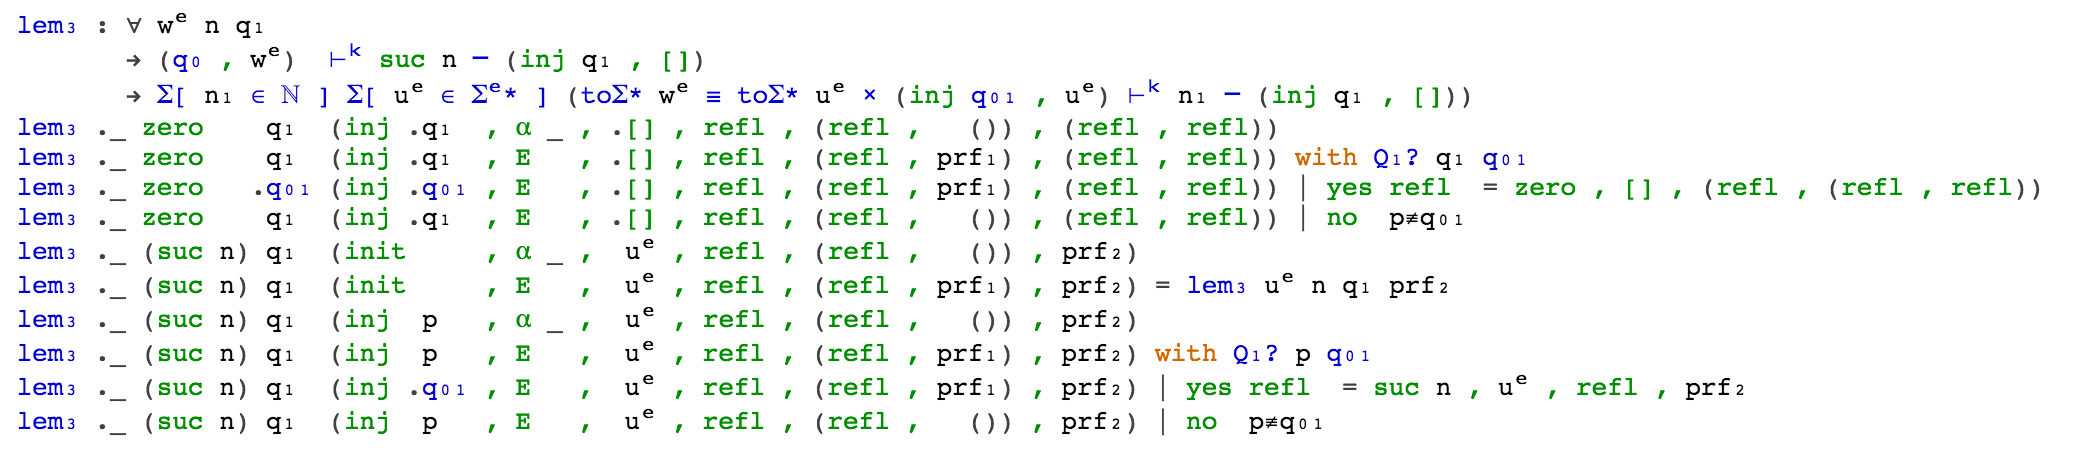
\includegraphics[width=\textwidth]{code} \end{center}

\par The above code is a proof that if \mb{w^e} can take \mb{q_0} to
another state \mb{inj\ q_1} in an \(\epsilon\)-NFA translated from a
regular expression \mb{e^*}, then there exists a number \mb{n_1} and
an \(\epsilon\)-string \mb{u^e} that will take \mb{inj\ q_{01}} to \mb{inj\ q_1} where
\mb{q_{01}} is the start state of \mb{e} and \mb{q_1} is a state in
\mb{e}. There are several techniques used in the proof; for example,
induction on natural numbers and case analysis on state comparison. However, by
just looking at the function body, the proving process can hardly be
understood. Therefore, in general, a computer proof is very inadequate on
this purpose and thus an outline of the proof in natural language is
still necessary. 

\paragraph{} Although computer proof seems to be unreadable, the advantages
are still impressive. For example, a group
of mathematicians may need months to validate a very long piece of
proof, but a computer proof may only need days to
compile. ... [ more ]


\subsubsection{Easiness or difficulty in the process of formalisation}
\par As a computer science student without a strong mathematical
background, I find it not very difficult to do the
formalisation as there are many similarities between writing codes and writing
proofs; for example, pattern matching compare to case analysis and
recursive function compare to mathematical induction. Furthermore, Agda is convenient
to use for its interactive features. The features allow us to know
what is happening inside the proof body by showing the goal and all the
elements in the proof. Also, many theorems can be automatically proved
by Agda. 
\par On the other hand, most of the
proof assistants based on dependent types support only primitive or
structural recursion. Many algorithms may be very difficult to
implement under this limitation. For example, the usual algorithm that
is used to compute the \(\epsilon\)-closure for a state \(q\) is as follow:
\begin{enumerate}[nolistsep]
  \item put \(q\) into a subset \(S\), i.e. \(S = \{q\}\)
  \item for every state \(p\) in \(S\), if another state \(r\) is
    reachable from \(p\) with an \(\epsilon\), i.e. \(r \in
        \delta (p,\ \epsilon)\), then put \(r\) into \(S\). 
  \item loop (2) until no new elements is added to \(S\)
  \item the resulting subset \(S\) is the $\epsilon$-closure of \(q\)
\end{enumerate}

\par This kind of algorithms cannot be implemented directly without
modifications. ... [ more ]


\subsubsection{Computer-aided verification and testing}
\par The most common way to verify a program is via testing. However,
no matter how sophisticated the design of the test cases is, the
program still cannot be proved to be 100\% correct. On the other
hand, total correctness can be achieved by proving the specifications
of a program. Already in 1997, Necula \cite{necula1997} has raised the
notion of \textit{Proof Carrying code}. The idea is to accompany
program with several proofs that proves the program specifications
within the same platform. In fact, there is already an
extraction mechanism \cite{letouzey2008} in Coq that allows us to
extract proofs and functions in Coq into Ocaml, Haskell or Scheme
programs. 

\par ... [ programming logic in concurrency, distributive systems,
cloud ] 